%!TEX root = ../bdr.tex
\chapter{Верстування текстової частини роботи}
А це просто текст...

Порожній рядок означає, що це був абзац

%\textbf{Lorem Ipsum is simply dummyl}  text of the printing and typesetting industry. Lorem Ipsum has been the industry's standard dummy text ever since the 1500s, when an unknown printer took a galley of type and scrambled it to make a type specimen book. It has survived not only five centuries, but also the leap into electronic typesetting, remaining essentially unchanged. It was popularised in the 1960s with the release of Letraset sheets containing Lorem Ipsum passages, and more recently with desktop publishing software like Aldus PageMaker including versions of Lorem Ipsum. 
\lipsum[2-4]

А це ненумерований список:
\begin{itemize}
\item Зелений;
\item Жовтий;
\item Білий.
\end{itemize}

А це нумерований список:
\begin{enumerate}
\item Колір
      \begin{enumerate}
      \item Зелений;
      \item Жовтий;
      \item Білий.
      \end{enumerate}	
\item Температура
      \begin{enumerate}
      \item Теплий;
      \item Холодний.
      \end{enumerate}
\end{enumerate}
 

\section{Рисунки}

Вставка рисунків робиться дуже просто:

\begin{figure}[h]
\caption{Опис рисунку}
\end{figure}

Далі можна вставити і сам рисунок (рис. \ref{fig:tux}). Він має бути у графічному файлі ({*}.jpg, {*}.png тощо). 

\begin{figure}[h]
 \centering
\includegraphics{img/Tux.png}
 \caption{Пінгвін}
 \label{fig:tux}
\end{figure}

Рисунок можна винести і в додаток (додаток \ref{apdx:text}), \label{linkpage} а посилання на нього залишити в основній частині роботи (рис. \ref{apdxfig:tux}).
Можна вручную вставляти картинки і прописувати кожний параметр.
Параметр width визначає ширину рисунку. У цьому випадку вона дорівнюватиме ширині текста \verb|\textwidth|. Замість \verb|\textwidth| можна вказати значення від 0.1 до 1. \verb|\label| потрібна для того, щоби потім можна було послатись на цю картинку, як тут.

\begin{figure}[!htb]
 \centering
 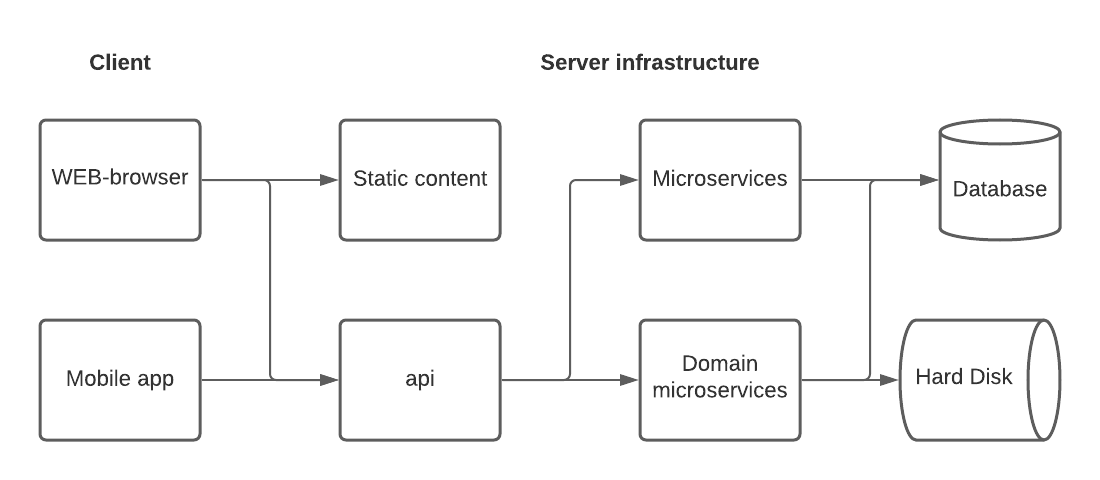
\includegraphics[width=0.8\textwidth]{img/fig1.png}
 \caption{Використовуйте Rich Text}
 \label{fig:fig1}
\end{figure}

\section{Таблиці}
Таблиці  - це складний об'єкт. Тому всі параметри треба прописувати вручну

\begin{table}[h!]
\centering
\begin{tabular}{|c|c|c|c|} 
 \hline
 Стопець1 & Стопець2 & Стопець3 & Стопець4 \\ [0.5ex] 
 \hline
 \multirow{3}{5em}{Декілька рядків} & 6 & 87837 & 787 \\ 
  &  7 & 78 & 5415 \\
   & 545 & 778 & 7507 \\
   & 545 & 18744 & 7560 \\
   & 88 & 788 & 6344 \\ [1ex] 
 \hline
\end{tabular}
\caption{Приклад роботи з таблицею}
\label{table:1}
\end{table}

\begin{table}[h]
	\caption{\label{table:2}Функціональна залежність параметрів ...}
	%\label{table:2}
	\begin{tabular}{|c|c|c|}
		\hline 
		Індекс & Показник 1 & Показник 2\tabularnewline
		\hline 
		\hline 
		1 & 2 & 3\tabularnewline
		\hline 
		4 & 5 & 6\tabularnewline
		\hline 
	\end{tabular}
\end{table}

Для табл. \ref{table:2} вже можете побачити легенду, яка на відміну від рисунків розташована зверху.

Великі таблиці можна повертати на 90 градусів:

%\begin{sidewaystable}
%	\centering{}
%	\caption{Набір компонентів.}
%	\begin{tabular}{|c|>{\raggedright}p{0.25\columnwidth}|>{\centering}p{0.15\columnwidth}|>{\centering}p{0.1\columnwidth}|}
%	\hline 
%	№ & Компонент  & Маса & К-сть\tabularnewline
%	\hline 
%	\hline 
%	1 & Компонент А & 12.8 & 100\tabularnewline
%	\hline 
%	2 & Компонент Б & 7.88 & 12\tabularnewline
%	\hline 
%	3 & Компонент В & 83.89 & 44\tabularnewline
%	\hline 
%	\end{tabular}
%\end{sidewaystable}

Більше про таблиці можна прочитати \href{https://www.overleaf.com/learn/latex/Tables}{тут}.

%\clearpage{}

\section{Формули...}

Формули, що входять до бакалврської роботи, нумерують в межах розділу. Номер формули складається з номера розділу та порядкового номера формули, розділених крапкою. Номер формули розташовують з правого боку на рівні формули в круглих дужках. По\-си\-лан\-ня в тексті на номер формули дають в дужках, наприклад, «... за формулою (\ref{eq:explan})». За необхідності вказують одиницю вимірювання, беручи її в квадратні дужки

\begin{equation}
\label{eq:explan}
I = \frac{U}{R}~[A].
\end{equation}

Числову підстановку і розрахунок виконують з нового рядка не нумеруючи. Одиницю вимірювання беруть в круглі дужки. Наприклад,

$$I = \frac{220}{100}~(\text{А}).$$

Розмірність одного й того ж параметра в межах документа має бути однаковою. Якщо формула велика, то її можна переносити в на\-ступ\-ні рядки. Перенесення виконують тільки математичними знаками, повторюючи знак на початку наступного рядка. При цьому знак мно\-жен\-ня «$\cdot$» замінюють знаком «$\times$».


\begin{align}
\label{xt:eq}
y(t) &= \frac{1}{{\rho}\,{S}\,{C_{f}}\,\sin\alpha}\Big(\ln\Big(\frac{1}{1962\,m}\Big(10\,v_0\sqrt{\rho\,S\,C_f\,\sin^3\alpha}\,\times \nonumber\\  &\times\cos\Big(\frac{3\,t\,\sqrt{218\,\rho\,S\,C_f\,\sin\alpha}}{20\,\sqrt{m}}\Big)\Big)^2\Big)\,m\Big).
\end{align}


Пояснення символів та числових коефіцієнтів наводять під формулою. Пояснення кожного символа подається з нового рядка в тій послідовності, в якій символи зустрічаються в формулі. Перший рядок пояснення починається зі слова «де» без двокрапки після нього.

\begin{equation}
T = 2\pi\sqrt{\frac{m}{k}}, 
\end{equation}

\begin{explanation}
\fitem $k$ -- коефіцієнт жорсткості пружини; 
\item $m$ -- маса тягарця.
\end{explanation}

Формула є частиною речення, тому до неї застосовують такі ж правила граматики, як і до інших членів речення. Якщо формула зна\-хо\-дить\-ся в кінці речення, то після неї ставлять крапку. 

Вставляти в текст можна формули будь-якої складності, як наприклад:

\begin{equation}
	\text{f=}\sqrt[12]{\sum\left(\beta*\xi\right)*\frac{z}{\arctan(123)}}*\top f(z)
\end{equation}


Формули з нумерацією    
\begin{equation}
    f(x)=\frac{x}{1+x^2}
\end{equation}

Ще одна формула    
\begin{equation}
    x^n + y^n = z^n
\end{equation}
    
А так прописуються формули, де нумерація не потрібна \(x^2 + y^2 = z^2\).

Другий спосіб - це вставити формулу між символам долара: $x^2 + y^2 = z^2$. 

\section{Формули без нумерації. Дроби.}
Для відтворення дробей в рядку, наприклад \(\frac{3x}{2}\), можна встановити інший стиль:
    \( \displaystyle \frac{3x}{2} \).
Це також працює і у зворотньому напрямку:
    \[ f(x)=\frac{P(x)}{Q(x)} \ \ \textrm{та}
    \ \ f(x)=\textstyle\frac{P(x)}{Q(x)} \]

\section{Інтеграли}
Інтеграл \(\int_{a}^{b} x^2 dx\) всередені тексту.
    \medskip
І той самий інтеграл між рядками:
    \[
    \int_{a}^{b} x^2 \,dx
    \]
    
Детальніше можна прочитати 
\href{https://www.overleaf.com/learn/latex/Integrals,_sums_and_limits#Integrals}{тут}.

\section{Суми і добутки}
Читати 
\href{https://www.overleaf.com/learn/latex/Integrals,_sums_and_limits#Sums_and_products}{тут}.

\section{Межі}
    
    Межа \(\lim_{x\to\infty} f(x)\) всередені тексту.
    І між рядками:
    \[
    \lim_{x\to\infty} f(x)
    \]

\section{Символи}
$\alpha A$ - грецькі,  $ \lambda; \Lambda$ - физичні величины=и, $\exists; \forall$ - логічні символм\\
За \href{https://www.overleaf.com/learn/latex/List_of_Greek_letters_and_math_symbols}{цим посиланням} можна одержати інформацію про інші символи. 
А \href{https://www.overleaf.com/learn/latex/Operators}{тут} - математичні оператори.

\section{Зноски, примітки та інш.}
У тексті зручно робити різноманітні зноски та примітки. Для цього їх достатньо встановити у необхідному місці, а форматування зробить свою потужну роботу. Ось приклад зноски, що розташується знизу \footnote{Це тест до зноски 1}. 

\section{LaTeX Wiki}
 Повне введення у LaTeX читайти \href{https://www.texlive.info/CTAN/info/lshort/russian/lshortru.pdf}{тут}.




